%Use one of the two documentclass lines depending on aspect ratio needed
% for 4x3 aspect ratio slides
%\documentclass{beamer}
%for 16x9 (modern wide screen) aspect ratio slides
\documentclass[aspectratio=169]{beamer}
\usepackage{tikz}
\usetikzlibrary{positioning}
% Oxford Maths theming
\usetheme{oxfordmaths}

% Set author etc info
\title[Onda sísmica con ML] %short version of title for slide footer
{Propagación de Onda Sísmica Usando Aprendizaje Automático} %full title for titlepage
\author{Oscar  Rincón}
\institute{Asignatura: Ecuaciones de la Física Matemática}
\date[5 Marzo 2025]  %short date for slide footer
{Universidad Nacional de Colombia sede Medellín\\Marzo 2025} %main date for title page,
                        %can overload it to show say 'Conference X, Date Y'


%% Now for the actual slides %%
\begin{document}

\begin{frame}[plain]
  \titlepage
\end{frame}

\begin{frame}
  \frametitle{Contenido}
{\Large   
  \begin{enumerate}\setlength{\itemsep}{1cm} % Ajusta el espacio entre ítems
  
  \item \hyperlink{onda}{Modelado de propagación de onda}
  \item \hyperlink{ml}{Métodos basados en Aprendizaje Automático}
  \item \hyperlink{inversion}{Inversión de forma de onda completa}

  \end{enumerate}
}  
\end{frame}

\begin{frame}
 \hypertarget{onda}{}
 
{\huge \textcolor{oxfordblue}{\textbf{1.}} Modelado de propagación de ondas sísmicas}

\end{frame}



\begin{frame}
\frametitle{El crecimiento de la literatura relacionada con el aprendizaje automático y el modelado de propagación de ondas}  


\includegraphics[width=1.0\textwidth]{figs/literature_trend.pdf}

\end{frame}

\begin{frame}
\frametitle{Interés en las bibliotecas de aprendizaje automático} 

\centering
\includegraphics[width=1.0\textwidth]{figs/packages_python.pdf}

\end{frame}


\begin{frame}
\frametitle{Ecuaciones diferenciales parciales}

Consideremos una PDE general definida sobre un dominio \( \Omega \) con límite \( \Gamma \):

\[
N[u(x, t), \lambda] = f(x,t), \quad x \in \Omega, \quad t \in [0, T] .
\]

%Donde:

\begin{itemize}
    \item \( N \) es un operador diferencial parametrizado por \( \lambda \). 
    \item \( u(x, t) \) es la solución desconocida.
    \item \( \Omega \) denota el dominio físico. 
    \item \( f(x, t) \) es un término fuente. 
\end{itemize}

\end{frame}

\begin{frame}
\frametitle{Ecuación de onda}

La ecuación de onda escalar (acústica) se utiliza ampliamente para estudiar las ondas sísmicas:

\[
\frac{\partial^2 u}{\partial t^2} - c^2 \Delta u = f(x, t),
\]

%donde el operador laplaciano está definido como:
 

%Los términos en la ecuación representan:

\begin{itemize}
    \item \(\Delta = \sum_{i=1}^{n} \frac{\partial^2}{\partial x_i^2}\).
    \item \( u(x, t) \) es la presión de las ondas generadas.
    \item \( f(x, t) \) es un término fuente que describe la fuerza y duración de la fuente.
\end{itemize}

\end{frame}

\begin{frame}
\frametitle{Modelado directo e inverso aplicado a la ecuación de onda}



\hspace{-1cm}
\makebox[\linewidth][l]{ % 'l' alinea a la izquierda
    \includegraphics[width=1.1\textwidth]{figs/escheme_inverse_problem.pdf}
}

\end{frame}

\begin{frame}
   \hypertarget{ml}{}
{\huge \textcolor{oxfordblue}{\textbf{2.}} Métodos basados en Aprendizaje Automático}


\end{frame}

\begin{frame}
\frametitle{Teorema de Aproximación Universal}

\begin{quote}
    Una red neuronal con una sola capa oculta y un número finito de neuronas puede aproximar cualquier función continua dada una función de activación apropiada.
\end{quote}

\vspace{0.5cm}
 
\centering
\begin{tikzpicture}[
    neuron/.style={circle, draw=oxfordblue, minimum size=0.7cm, inner sep=0pt},
    >=stealth
]

% Neurona de entrada
\node[neuron] (x) { $x$ };

% Neuronas ocultas
\node[neuron, right=1.8cm of x, yshift=1cm] (h1) { $n_1$ };
\node[neuron, right=1.8cm of x] (h2) { $n_2$ };
\node[below=0.25cm of h2] (hdots) { $\vdots$ };
\node[neuron, right=1.8cm of x, yshift=-2cm] (hm) { $n_m$ };

% Neurona de salida
\node[neuron, right=2.2cm of h2] (y) { $\hat{f}$ };

% Texto "≈ f" a la derecha de la salida
\node[right=0.1cm of y] {$\approx f$};

% Conexiones entrada -> capa oculta
\foreach \j in {1,2,m}
    \draw[->] (x.east) -- (h\j.west);

% Conexiones capa oculta -> salida
\foreach \j in {1,2,m}
    \draw[->] (h\j.east) -- (y.west);

\end{tikzpicture}

\end{frame}


\begin{frame}
\frametitle{Ejemplo de Aproximación de funciones con redes neuronales}

Vamos a aproximar la siguente función:

\[
f(x)  x^{3} + x^{2} - x - 1
\]

Con una red de una capa:

\[
\hat{f}(x) = \sum_{i=1}^{5} w^{(2)}_i \cdot \tan^{-1} \left( w^{(1)}_i x + b^{(1)}_i \right) + b^{(2)}
\]



\end{frame}
 
\begin{frame}
\frametitle{Aproximación de funciones con redes neuronales}

Para una red neuronal con múltiples capas ocultas, la aproximación de una función \( u(x) \) se expresa como:

\[
\text{NN}(x; \theta) = W_L \sigma_{L-1} \left( W_{L-1} \sigma_{L-2} \left( \dots \sigma_1(W_1 x + b_1) \dots \right) + b_{L-1} \right) + b_L \approx u(x)
\]

%donde:

\begin{itemize}
    \item \( L \) es el número total de capas de la red.
    \item \( W_\ell \) y \( b_\ell \) son los pesos y sesgos de la capa \( \ell \), para \( \ell = 1, \dots, L \).
    \item \( \sigma_\ell \) es la función de activación de la capa \( \ell \).
    \item \( \theta = \{ W_\ell, b_\ell \}_{\ell=1}^{L} \) representa el conjunto de parámetros de la red.
    \item \( \text{NN}(x; \theta) \) es la salida de la red neuronal, que busca aproximar la función \( u(x) \).
\end{itemize}

\end{frame}




\begin{frame}
\frametitle{Función de pérdida para la optimización}

La función de pérdida a optimizar es:

\[
L = \frac{1}{N} \sum_{i=1}^{N} \left\| \text{NN}(x_i, \theta) - u(x_i) \right\|
\]

%donde:

\begin{itemize}
    \item \( \text{NN}(x_i, \theta) \) es la salida de la red neuronal.
    \item \( u(x_i) \) es la función objetivo que queremos aproximar.
    \item \( N \) es el número de datos conocidos.
\end{itemize}

\end{frame}

\begin{frame}
\frametitle{Optimización mediante descenso de gradiente}

El \textcolor{oxfordblue}{método de descenso de gradiente} se expresa como:

\[
\theta^{(i+1)} = \theta^{(i)} - \alpha \nabla_{\theta} L(\theta)
\]

%donde:

\begin{itemize}
    \item \( \theta \) representa los parámetros a optimizar.
    \item \( L(\theta) \) es la función de pérdida.
    \item \( \alpha \) es la tasa de aprendizaje.
\end{itemize}

\end{frame}


\begin{frame}\frametitle{La arquitectura básica de las redes neuronales artificiales}

\hspace{-1cm}
\makebox[\linewidth][l]{ % 'l' alinea a la izquierda
    \includegraphics[width=1.1\textwidth]{figs/escheme_nn.pdf}
}

\end{frame}

\begin{frame}
\frametitle{Aproximación de una PDE sin datos mediante una Red Neuronal}

Supongamos que queremos aproximar la solución de una ecuación en derivadas parciales (PDE) sin datos:  

\[
u(x, t)_{tt} - c^2 \Delta u(x, t) = f(x, t),
\]

donde aproximamos la solución mediante una red neuronal:  

\[
u(x, t) \approx \text{NN}(x, t; \theta),
\]
\[
u_{tt}(x, t) \approx \text{NN}_{tt}(x, t; \theta),
\]
\[
\Delta u(x, t) \approx \Delta \text{NN}(x, t; \theta).
\]

Sustituyendo estas aproximaciones en la ecuación diferencial, obtenemos:  

\[
\text{NN}(x, t)_{tt} - c^2 \Delta \text{NN}(x, t) - f(x, t) = 0.
\]

Esto permite aproximar la PDE mediante una red neuronal.
\end{frame}

\begin{frame}
\frametitle{Planteamiento de la función de perdida de una PDE}

Podemos aproximar la ecuación en derivadas parciales (PDE) mediante una red neuronal:

\[
\text{NN}(x, t)_{tt} - c^2 \Delta \text{NN}(x, t) - f(x, t) = 0.
\]

Para optimizar la solución, definimos una función de pérdida que mida el error de la red neuronal respecto a la ecuación diferencial:

\[
L_{\text{PDE}} = \frac{1}{N_{\text{PDE}}} \sum_{i=1}^{N_{\text{PDE}}} 
\left\| \text{NN}(x_i, t_i)_{tt} - c^2 \Delta \text{NN}(x_i, t_i) - f(x_i, t_i) \right\|,
\]

para \( x \in \Omega \), \( t \in [0, T] \).

\end{frame}



\begin{frame}\frametitle{Esquema de redes neuronales basado en la física aplicado a la ecuación de onda}


\hspace{0.5cm}
 \includegraphics[width=0.85\textwidth]{figs/escheme_pinns.pdf}
 

\end{frame}

\begin{frame}
 

\small % Reduce el tamaño del texto
\textcolor{oxfordblue}{\textbf{Algoritmo de redes neuronales informadas por física}}\\

\

\noindent\texttt{\textbf{Entradas:} Conjunto de puntos de muestreo del dominio \( \Omega \) con la EDP gobernante, condiciones iniciales y condiciones de frontera.\\ 
\textbf{Salidas:} Aproximación de la solución \( u(\mathbf{x}, t) \),  parámetros estimados \( \lambda \)\\ 
1. Inicializar parámetros: \( \theta \) (y \( \lambda \) si se infiere). \\
2. Definir tolerancia e iteraciones máximas: \(\text{tol} > 0\), \(\text{maxiter} > 0\). \\
3. Inicializar tasa de aprendizaje: \( \alpha_k \). \\
4. Para cada método en \{Adam, L-BFGS\}: \\
\hspace{5mm} \( k = 0 \) \\
\hspace{5mm} \textbf{While} \( k < \text{maxiter} \) y \( L(\theta^{(k)}) > \text{tol} \) \textbf{hacer}: \\
\hspace{10mm} - Evaluar \( u(x, t; \theta^{(k)}) \). \\
\hspace{10mm} - Calcular la función de pérdida: \\
\hspace{15mm} \( L(\theta^{(k)}) = L_{\Omega} + L_{\Gamma} + L_{\text{IC}} \). \\
\hspace{10mm} - Actualizar parámetros: \\
\hspace{15mm} \( \theta^{(k+1)} = \theta^{(k)} - \alpha_k \nabla L(\theta^{(k)}) \). \\
\hspace{10mm} - Incrementar \( k = k + 1 \). \\
\hspace{5mm} \textbf{End While}. \\
}

\end{frame}

\begin{frame}
\frametitle{Problemas inversos con redes neuronales informadas por física}

La función de pérdida para resolver un problema inverso es:

\[
L = \frac{1}{N_{\text{PDE}}} \sum_{i=1}^{N_{\text{PDE}}} \left\| \frac{\partial^2 \text{NN}(x, t)}{\partial t^2} - c^2 \Delta \text{NN}(x, t) - f(x, t) \right\|
\]

\[
+ \frac{1}{N_d} \sum_{i=1}^{N_d} \left\| \text{NN}(x_i, \theta) - u(x_i) \right\|
\]

Si se dispone de datos adicionales, además de la solución de la PDE, se puede estimar el parámetro \( c^2 \).

\end{frame}


\begin{frame}
\frametitle{Aplicación de redes neuronales informadas por física en un problema inverso}

Consideremos las ecuaciones de Navier-Stokes en dos dimensiones:

\[
u_t + \lambda_1 (u u_x + v u_y) = -p_x + \lambda_2 (u_{xx} + u_{yy}),
\]
\[
v_t + \lambda_1 (u v_x + v v_y) = -p_y + \lambda_2 (v_{xx} + v_{yy}).
\]

%Donde:

\begin{itemize}
    \item \( u(t, x, y) \) es el componente \( x \) del campo de velocidad.
    \item \( v(t, x, y) \) es el componente \( y \) del campo de velocidad.
    \item \( p(t, x, y) \) es la presión del fluido.
    \item \( \lambda = (\lambda_1, \lambda_2) \) son los parámetros desconocidos a estimar.
\end{itemize}

Se dispone de valores de \( u(t, x, y) \), \( v(t, x, y) \) y \( p(t, x, y) \) en puntos aleatorios del dominio.

\end{frame}

\begin{frame}\frametitle{Esquema del problema inverso con redes neuronales informadas por física}

\centering
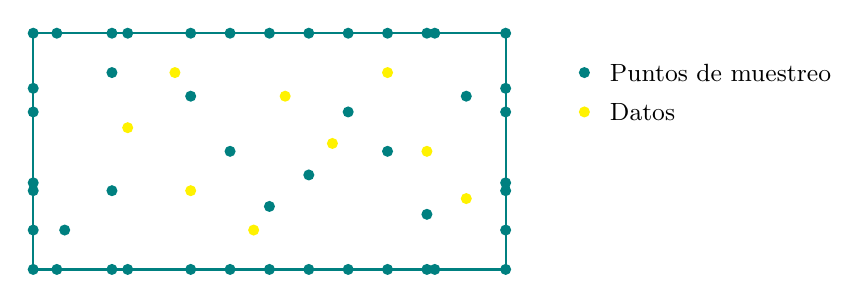
\begin{tikzpicture}

    % Dibujar el rectángulo
    \draw[thick, teal] (0,0) rectangle (6,3);
    
    % Puntos de muestreo (borde y dentro del dominio)
    \foreach \x in {0,0.3,1,1.2,2,2.5,3,3.5,4,4.5,5,5.1,6} {
        \foreach \y in {0,3} {
            \fill[teal] (\x,\y) circle (2pt);
        }
    }
    \foreach \y in {0.5,1,1.1,2,2.3} {
        \fill[teal] (0,\y) circle (2pt);
        \fill[teal] (6,\y) circle (2pt);
    }
    
    % Puntos de muestreo dentro del dominio
    \foreach \x/\y in {1/2.5, 2.5/1.5, 4/2, 3/0.8, 5.5/2.2, 2/2.2, 3.5/1.2, 5/0.7, 4.5/1.5,1,0.4/0.5} {
        \fill[teal] (\x,\y) circle (2pt);
    }

    % Puntos de datos dentro del dominio
    \foreach \x/\y in {1.2/1.8, 2/1, 3.8/1.6, 5/1.5, 4.5/2.5, 1.8/2.5, 2.8/0.5, 3.2/2.2, 5.5/0.9} {
        \fill[yellow] (\x,\y) circle (2pt);
    }

    % Leyenda
    \fill[teal] (7,2.5) circle (2pt);
    \node[right] at (7.2,2.5) {\small Puntos de muestreo};
    
    \fill[yellow] (7,2) circle (2pt);
    \node[right] at (7.2,2) {\small Datos};

\end{tikzpicture}
\end{frame}


\begin{frame}
   \hypertarget{inversion}{}
{\huge \textcolor{oxfordblue}{\textbf{3.}} Inversión de forma de onda completa}

\end{frame}

\begin{frame}
\frametitle{Inversión de Forma de Onda Completa (FWI)}

La inversión de forma de onda completa (FWI) es una técnica de imágenes sísmicas de alta resolución que utiliza la información completa de las ondas sísmicas para estimar los parámetros físicos del medio. 

\vspace{0.5cm}
\centering
\includegraphics[width=0.85\textwidth]{figs/fwi.pdf}

\vspace{0.2cm}
\begin{flushleft}
{\footnotesize
P. Jin et al., “An empirical study of large-scale data-driven full waveform inversion,” \textit{Scientific Reports}, vol. 14, no. 1, p. 20034, Aug. 2024, doi: \href{https://doi.org/10.1038/s41598-024-68573-7}{10.1038/s41598-024-68573-7}.}
\end{flushleft}

\end{frame}


\begin{frame}
\frametitle{Optimización en la Inversión de Forma de Onda Completa (FWI)}

El objetivo de la inversión de forma de onda completa (FWI) es minimizar la función de pérdida basada en mínimos cuadrados:

\[
L = \frac{1}{2} \left\| d_{\text{calc}}(m) - d_{\text{obs}} \right\|^2
\]

Donde:
\begin{itemize}
    \item \( m \) representa los parámetros del modelo a determinar.
    \item \( \mathbf{x} = (x, y, z) \) son las coordenadas espaciales.
    \item \( d_{\text{obs}} \) son los datos sísmicos observados.
    \item \( d_{\text{calc}} \) son los datos calculados a partir del modelo.
\end{itemize}

Los parámetros del modelo, en este caso la velocidad de propagación en el medio, son optimizados iterativamente mediante el siguiente esquema de actualización:

\[
m^{(k+1)} = m^{(k)} - \alpha_k \nabla L(m^{(k)})
\]

\end{frame}

\begin{frame}

\includegraphics[width=1.0\textwidth]{figs/fwi_1.pdf}

\begin{flushleft}
{\footnotesize
M. A. Londoño and F. J. Rodríguez-Cortés, “Application of an RBF-FD solver for the Helmholtz equation to full-waveform inversion,” Jan. 23, 2022, arXiv: arXiv:2201.09378.}
\end{flushleft}

\end{frame}

\begin{frame}

\includegraphics[width=0.8\textwidth]{figs/fwi_2.pdf}



\begin{flushleft}
{\footnotesize
M. A. Londoño and F. J. Rodríguez-Cortés, “Application of an RBF-FD solver for the Helmholtz equation to full-waveform inversion,” Jan. 23, 2022, arXiv: arXiv:2201.09378.}
\end{flushleft}

\end{frame}

\begin{frame}\frametitle{Conclusiones}

\begin{itemize}
    \item Las redes neuronales informadas por la física permiten integrar tanto datos experimentales como el conocimiento matemático del sistema para resolver problemas inversos de manera eficiente.  
    \item Estas redes representan una alternativa prometedora para la implementación del método de inversión de onda completa, mejorando la precisión y robustez en la estimación de parámetros del medio.  
    \item En general, se busca aprovechar herramientas modernas de aprendizaje automático para abordar diversos problemas en ciencia e ingeniería, optimizando procesos y reduciendo costos computacionales.  
\end{itemize}

\end{frame}


\begin{frame}

\end{frame}

\end{document}
